\documentclass[xcolor]{beamer}

% Pacotes Principais -----------------------------------------------------------
\usepackage[portuges,brazil]{babel}
\usepackage[utf8]{inputenc}

% Formatação de capítulos ------------------------------------------------------
%\usepackage[Sonny]{fncychap}
%\usepackage{fncychap}
\usepackage{capitulos}

% Figuras e Imagens ------------------------------------------------------------
\usepackage{graphicx}
% Figuras lado a lado
\usepackage{epsfig}
\usepackage{subfigure}

% Utilizar H para inserir as imagens REALMENTE onde eu desejo
\usepackage{float}

% Fontes -----------------------------------------------------------------------
\usepackage[T1]{fontenc}
\usepackage{pslatex}

% Simbolos ---------------------------------------------------------------------
\usepackage{textcomp}
\usepackage{bbding}

% Tabelas ----------------------------------------------------------------------
%\usepackage{multicol}
\usepackage{multirow}
% Colorir a tabela
\usepackage{colortbl}
% Pacote hhline corrige os bugs das linhas que não aparecem com o colortbm
\usepackage{hhline}
% Tabelas com colunas de largura auto ajustável
\usepackage{tabularx}
% Notas de rodapé em tabelas (Pode-se usar o ambiente longtable também -
% Pesquisar exemplo com longtable)
\usepackage{threeparttable}
% Tabelas grandes
\usepackage{supertabular}

% Glossário --------------------------------------------------------------------
\usepackage[portuguese,noprefix]{nomencl}
\usepackage{makeglo}

% Outros pacotes ---------------------------------------------------------------
\usepackage{noitemsep}

% Comentários em bloco
\usepackage{verbatim}

% Hiperlinks
\usepackage{hyperref}

% Orientação de página
\usepackage{lscape}

% utilitários matemáticos
\usepackage{amsmath}
\usepackage{icomma}

% Evita o problema "too many unprocessed floats", colocando os campos
% 'flutuantes' em suas respectivas seções
\usepackage[section]{placeins}

% Referências ------------------------------------------------------------------
\usepackage[abbr]{harvard}	% As chamadas são sempre abreviadas
\harvardparenthesis{square}	% Colchetes nas chamadas
\harvardyearparenthesis{round}	% Parêntesis nos anos das referências
\renewcommand{\harvardand}{e}	% Substituir "&" por "e" nas referências

% Comandos gerais --------------------------------------------------------------
\newcommand{\titulo}{Sistemas de Tempo Real}
\newcommand{\autor}{Diogo Leite Rebouças}

% Configuração da fonte
%\renewcommand{\familydefault}{\sfdefault}

% Margens ----------------------------------------------------------------------
\setlength{\oddsidemargin}{3.5cm}
\setlength{\evensidemargin}{2.5cm}
\setlength{\textwidth}{15cm}
\addtolength{\oddsidemargin}{-1in}
\addtolength{\evensidemargin}{-1in}

\setlength{\topmargin}{2.0cm}
\setlength{\headheight}{1.0cm}
\setlength{\headsep}{1.0cm}
\setlength{\textheight}{22.7cm}
\setlength{\footskip}{1.0cm}
\addtolength{\topmargin}{-1in}

% Glossário --------------------------------------------------------------------
\makeglossary

% Capítulos --------------------------------------------------------------------
% Não aparecer o número na primeira página dos capítulos
\newcommand{\mychapter}[1]{\chapter{#1}\thispagestyle{empty}}
\newcommand{\mychapterstar}[1]{\chapter*{#1}\thispagestyle{empty}}

% Comandos matemáticos ---------------------------------------------------------
% Implicação em fórmulas
\newcommand{\implica}{\quad\Rightarrow\quad} %Meio de linha
\newcommand{\implicafim}{\quad\Rightarrow}   %Fim de linha
\newcommand{\tende}{\rightarrow}

% Fração com parenteses
\newcommand{\pfrac}[2]{\parent{\frac{#1}{#2}}}

% Transformada de Laplace e transformada Z
\newcommand{\lapl}{\pounds}
\newcommand{\transfz}{\mathcal{Z}}

% Sequências
\newcommand{\sequencia}[4]{$#1_{#2}$, $#1_{#3}$, \ldots, $#1_{#4}$}

% Outros ----------------------------------------------------------------------
\newcommand{\chave}[1]{\left\{#1\right\}}
\newcommand{\colchete}[1]{\left[#1\right]}
\newcommand{\parent}[1]{\left(#1\right)}

\newcommand{\rhoagua}{\rho_{\tiny \text{\tiny H}_2\text{\tiny O}}}

\let\D\displaystyle
\newcommand{\reg}{\textsuperscript{\textregistered}}
\newcommand{\soft}{\textit{software}}
\newcommand{\Soft}{\textit{Software}}

% Imagens exportadas pelo gnuplot ----------------------------------------------
\graphicspath{{imgs/eps/}}


% Temas ========================================================================
\mode<presentation>
{
%\usetheme[blue,noshadow]{Trondheim}
%\usetheme[blue,minimal]{Trondheim}
\usetheme[blue,compress,numbers,nonav]{Trondheim}
%\usetheme[sand,compress,numbers,nonav,innovation]{Trondheim}
%\usetheme{default}

% Inner ........................................................................
%\useinnertheme{default}
%\useinnertheme{rounded}
%\useinnertheme{inmargin}
%\useinnertheme{rectangles}
\useinnertheme{circles}

% Outer ........................................................................
%\useoutertheme{default}
%\useoutertheme{infolines}
%\useoutertheme{miniframes}
%\useoutertheme{ntnu}
%\useoutertheme{shadow}
%\useoutertheme{sidebar}
%\useoutertheme{smoothbars}
%\useoutertheme{smoothtree}
%\useoutertheme{split}
%\useoutertheme{tree}

% Color ........................................................................
%\usecolortheme{albatross}
%\usecolortheme{beaver}
%\usecolortheme{beetle}
%\usecolortheme{crane}
%\usecolortheme{default}
%\usecolortheme{dolphin}
%\usecolortheme{dove}
%\usecolortheme{fly}
%\usecolortheme{lily}
%\usecolortheme{ntnublue}
%\usecolortheme{ntnuold}
%\usecolortheme{orchid}
%\usecolortheme{rose}
%\usecolortheme{seagull}
%\usecolortheme{seahorse}
%\usecolortheme{sidebartab}
%\usecolortheme{structure}
%\usecolortheme{whale}
%\usecolortheme{wolverine}
}

% Configuração da página inicial ===============================================
\title[Sistemas Multimídia]
{
    Sistemas Multimídia
}
\subtitle{Introdução ao Sinal}
\author[Diogo Leite Rebouças]
{
    Diogo Leite Rebouças\\
    {\tt diogolr@gmail.com}
}
\institute
{
    Universidade do Estado do Rio Grande do Norte\\
    Departamento de Informática
}
\date{\today}
\pgfdeclareimage[width=1.5cm,interpolate=true]{ntnulogotext}{imgs/uern}

% Inicio do documento ==========================================================
\begin{document}

\maketitle
%\compressedtitle

% Logo somente após a capa
\logo{
\includegraphics[width=0.75cm]{imgs/uern}}

% Sumário ......................................................................
\begin{frame}
    \frametitle{Sumário}
    \tableofcontents
\end{frame}

\section{Introdução}
\subsection{Informação e Sinal}
\begin{frame}
    \frametitle{Informação e sinal}

    Início do desenvolvimento de sistemas (sistemas operacionais, redes de
    comunicação, sistemas de processamento)

    \begin{itemize}
        \item Processamento e comunicação de dados textuais
    \end{itemize}

    Evolução tecnológica

    \begin{itemize}
        \item Aumento do poder de processamento
        \item Aumento da capacidade de armazenamento
        \item Processar somente dados textuais \implica Matar lagartixa com
              bazuca
    \end{itemize}
\end{frame}

\begin{frame}
    \frametitle{Informação e sinal}

    Surgimento de novos tipos de representação da informação:

    \begin{itemize}
        \item Arquivos de Áudio
        \item Arquivos de Imagem
        \item Arquivos de Vídeo
        \item Arquivos de Áudio e Vídeo
    \end{itemize}

    Mas o que seria tudo isso se não pudéssemos ``entender'' o significado das
    coisas?

    \vspace{0.25cm}

    Os 5 sentidos humanos:

    \begin{itemize}
        \item \alert{Visão}
        \item Tato (tecnologias emergentes \ldots)
        \item Olfato (poucas coisas \ldots)
        \item \alert{Audição}
        \item Paladar (não conheço, ainda \ldots)
    \end{itemize}
\end{frame}

\begin{frame}
    \frametitle{Informação e sinal}

    Esses sentidos são os conhecidos como {\it mídias de percepção}

    \vspace{0.25cm}

    Informações adquiridas são codificadas em estruturas denominadas {\it mídias
    de representação} ou, simplesmente, {\it mídias}

    \vspace{0.25cm}

    São exemplos de {\it mídias de representação} as mídias de texto, imagem,
    áudio e vídeo armazenadas em seus computadores

    \vspace{0.25cm}

    \obs{Não existe ainda correspondência biunívoca entre as mídias de percepção
         e mídias de representação}

    O que seria então sinal e o que seria informação?
\end{frame}

\begin{frame}
    \frametitle{Informação e sinal}

    \defin{{\bf Sinais} são ondas (físicas/eletromagnéticas) que podem ser
    transmitidos através de algum meio físico. A variação de alguma
    característica desse sinal (amplitude, frequência, largura de pulsos \ldots)
    corresponde à codificação da {\bf informação} a ser transmitida.}

    Objetivos da transmissão:

    \begin{itemize}
        \item Transmitir o sinal sem perda/deformação
        \item Decodificar o sinal transmitido
        \item Apresentar a informação
    \end{itemize}
    
    Problemas envolvidos:

    \begin{itemize}
        \item Distorção do sinal (atenuação, ruído, deformação)
        \item Perda de informação
        \item Limitações do meio de transmissão (banda passante)
    \end{itemize}
\end{frame}

\begin{frame}
    \frametitle{Informação e sinal}

    Qualidade do sinal x Qualidade da informação

    \vspace{0.25cm}

    Exemplo:

    \begin{itemize}
        \item Vídeo transmitido a 30 fps (padrão de TV)
        \item Vídeo transmitido a 10 fps (a cada 3 quadros 2 são perdidos)
    \end{itemize}

    O que aconteceria se estivéssemos transmitindo:

    \begin{itemize}
        \item Uma paisagem sem movimento (imagem estática) \implica Até mesmo só
              um quadro resolveria \ldots
        \item Transmissão esportiva \implica Movimentos bruscos, sem
              naturalidade
    \end{itemize}

    O que se pode concluir desse exemplo?
\end{frame}

\begin{frame}
    \frametitle{Informação e sinal}

    Sinal pode carregar muita informação redundante.

    \vspace{0.25cm}

    Técnicas para redução da redundância da informação (compressão e
    compactação) \implica Aulas posteriores \ldots
\end{frame}

\subsection{Representação da informação}

\begin{frame}
    \frametitle{Representação da informação}

    Início \implica Computadores processavam números e palavras

    \vspace{0.25cm}

    Representação dos números:

    \begin{itemize}
        \item Binários
        \item BCD -- {\it Binary Coded Decimal}
        \item IEEE 754 -- Ponto flutuante
    \end{itemize}

    Representação de dados alfanuméricos:

    \begin{itemize}
        \item ASCII
        \item UTF8
        \item EBCDIC
    \end{itemize}
\end{frame}

\begin{frame}
    \frametitle{Representação da informação}

    Introdução da representação gráfica

    \vspace{0.25cm}

    Tipos de representação de imagens:

    \begin{itemize}
        \item Vetorial
        \item Matricial (Bitmap Binário, Malha RGB, Malha RGBA)
    \end{itemize}

    Formato vetorial:

    \begin{itemize}
        \item Muito utilizada em modelagem geométrica
        \item Representação das imagens através de um conjunto de segmentos de
              retas/curvas
        \item Utilização de um plano de coordenadas (2D ou 3D)
        \item Utilização de características/atributos para cada elemento da
              imagem
    \end{itemize}
\end{frame}

\begin{frame}
    \frametitle{Representação da informação}

    Formato matricial (imagens estáticas):

    \begin{itemize}
        \item Imagens divididas em pequenas regiões (elementos de fotografia --
              {\it pixels -- picture elements})
        \item Cada \pixel \implica Informação codificada em cores (RGB,
              RGBA)
        \item Maior o número de bits \implica Mais informação pode ser
              armazenada \implica Cores mais ``reais''
    \end{itemize}

    Exemplo:

    \begin{itemize}
        \item Matriz $M \times N$ \implica $MN$ {\it pixels}
        \item RGB (8 bits/cor = 24 bits) \implica $24 MN$ bits necessários para
              representar a imagem
        \item Quantas cores podem ser representadas em cada \pixel?
    \end{itemize}
\end{frame}

\begin{frame}
    \frametitle{Representação da informação}

    \exemp
    {
        RGB = {\color{red!80!black}{8 bits}} + 
              {\color{green!80!black}{8 bits}} + 
              {\color{blue!80!black}{8 bits}} = 24 bits

        8 bits \implica 256 combinações

        \vspace{0.25cm}

        RGB = {\color{red!80!black}{256}} $\times$
              {\color{green!80!black}{256}} $\times$ 
              {\color{blue!80!black}{256}} = 16.777.216 cores distintas
    }

    Quanto menor o tamanho do \pixel:

    \begin{itemize}
        \item Coloração mais fiel à original
        \item Maior a matriz da imagem
    \end{itemize}

    Tamanho da matriz \implica {\it resolução geométrica}

    \vspace{0.25cm}

    Quantidade de bits utilizados \implica {\it resolução de cor}
    \vspace{0.25cm}
\end{frame}

\begin{frame}
    \frametitle{Representação da informação}

    Representação gráfica e textual \implica Representações digitais \implica
    {\it mídias discretas}

    \vspace{0.25cm}

    Fontes sonoras ou de vídeo \implica Representação real (sinais
    analógicos) \implica {\it mídias contínuas}

    \obs{Importante entender que qualquer tipo de informação (analógica ou
    digital) pode ser codificada em uma estrutura de dados (mídia de
    representação) digital. A transmissão da informação codificada pode ser
    analógica ou digital.}

    Transmissão digital \implica Recuperação do sinal transmitido mesmo na
    presença de falhas, distorções ou ruídos
\end{frame}

\section{Conversão de sinais}
\subsection{Conversão A/D}
\begin{frame}
    \frametitle{Conversão A/D}

    Em síntese \implica Transformação da mídia contínua em mídia discreta (mídia
    digital)

    \vspace{0.25cm}

    Teorema de Nyquist:

    \begin{itemize}
        \item Amostragem feita em $2W$ garante recuperação de sinal com banda
              passante $W$
   
              \vspace{0.25cm}
    
              \begin{figure}[htb]
              \centering
                  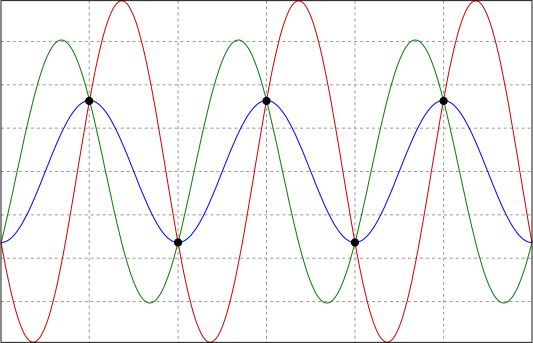
\includegraphics[width=0.45\textwidth]{imgs/nyquist}
              \end{figure}
        \item Armazenamento dos valores das amplitudes das amostras tomadas a
              cada $\frac{1}{2W}$
    \end{itemize}
\end{frame}

\begin{frame}
    \frametitle{Conversão A/D}

    Processo de amostragem

    \begin{itemize}
        \item Modulação por Amplitude de Pulsos ({\it Pulse Amplitude Modulation
              -- PAM}) \implica Modulação por Codificação de Pulsos ({\it Pulse
              Code Modulation -- PCM}) através da quantização ($n$ bits)
    \end{itemize}

    \begin{figure}[htb]
    \centering
        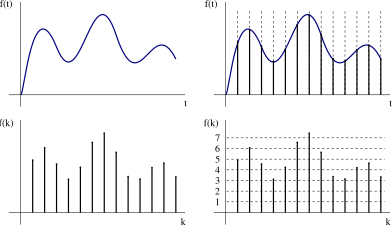
\includegraphics[width=0.8\textwidth]{imgs/pcm}
    \end{figure}

    \scriptsize
    Saída PCM: 101|110|100|011|\ldots

\end{frame}


\subsection{Conversão D/A}
\begin{frame}
    \frametitle{Conversão D/A}

    Em síntese \implica Transformação da mídia digital em mídia contínua
    (perceptível pelos sentidos humanos)

        %Segurador de Ordem Zero ({\it Zero Order Holder -- ZOH})

\end{frame}

\end{document}
